%% knit("our_lass_report_analysis.Rnw")

\documentclass[12pt]{article}\usepackage[]{graphicx}\usepackage[]{color}
%% maxwidth is the original width if it is less than linewidth
%% otherwise use linewidth (to make sure the graphics do not exceed the margin)
\makeatletter
\def\maxwidth{ %
  \ifdim\Gin@nat@width>\linewidth
    \linewidth
  \else
    \Gin@nat@width
  \fi
}
\makeatother

\definecolor{fgcolor}{rgb}{0.345, 0.345, 0.345}
\newcommand{\hlnum}[1]{\textcolor[rgb]{0.686,0.059,0.569}{#1}}%
\newcommand{\hlstr}[1]{\textcolor[rgb]{0.192,0.494,0.8}{#1}}%
\newcommand{\hlcom}[1]{\textcolor[rgb]{0.678,0.584,0.686}{\textit{#1}}}%
\newcommand{\hlopt}[1]{\textcolor[rgb]{0,0,0}{#1}}%
\newcommand{\hlstd}[1]{\textcolor[rgb]{0.345,0.345,0.345}{#1}}%
\newcommand{\hlkwa}[1]{\textcolor[rgb]{0.161,0.373,0.58}{\textbf{#1}}}%
\newcommand{\hlkwb}[1]{\textcolor[rgb]{0.69,0.353,0.396}{#1}}%
\newcommand{\hlkwc}[1]{\textcolor[rgb]{0.333,0.667,0.333}{#1}}%
\newcommand{\hlkwd}[1]{\textcolor[rgb]{0.737,0.353,0.396}{\textbf{#1}}}%

\usepackage{framed}
\makeatletter
\newenvironment{kframe}{%
 \def\at@end@of@kframe{}%
 \ifinner\ifhmode%
  \def\at@end@of@kframe{\end{minipage}}%
  \begin{minipage}{\columnwidth}%
 \fi\fi%
 \def\FrameCommand##1{\hskip\@totalleftmargin \hskip-\fboxsep
 \colorbox{shadecolor}{##1}\hskip-\fboxsep
     % There is no \\@totalrightmargin, so:
     \hskip-\linewidth \hskip-\@totalleftmargin \hskip\columnwidth}%
 \MakeFramed {\advance\hsize-\width
   \@totalleftmargin\z@ \linewidth\hsize
   \@setminipage}}%
 {\par\unskip\endMakeFramed%
 \at@end@of@kframe}
\makeatother

\definecolor{shadecolor}{rgb}{.97, .97, .97}
\definecolor{messagecolor}{rgb}{0, 0, 0}
\definecolor{warningcolor}{rgb}{1, 0, 1}
\definecolor{errorcolor}{rgb}{1, 0, 0}
\newenvironment{knitrout}{}{} % an empty environment to be redefined in TeX

\usepackage{alltt}
\usepackage{times}
\usepackage{hyperref}
\usepackage{natbib}
\hypersetup{pdfpagemode=UseNone} % don't show bookmarks on initial view
\hypersetup{colorlinks, urlcolor={blue}}

% revise margins
\setlength{\headheight}{0.0in}
\setlength{\topmargin}{0.0in}
\setlength{\headsep}{0.0in}
\setlength{\textheight}{8.65in}
\setlength{\footskip}{0.35in}
\setlength{\oddsidemargin}{0.0in}
\setlength{\evensidemargin}{0.0in}
\setlength{\textwidth}{6.5in}

\setlength{\parskip}{6pt}
\setlength{\parindent}{0pt}

\title{\emph{Our Lass} 70mm versus 80mm analysis}
\author{For discussion}
\date{}
\IfFileExists{upquote.sty}{\usepackage{upquote}}{}
\begin{document}



\maketitle

\section{Data}

Read the data in and make a few factor variables
\begin{knitrout}\footnotesize
\definecolor{shadecolor}{rgb}{0.969, 0.969, 0.969}\color{fgcolor}\begin{kframe}
\begin{alltt}
\hlkwd{library}\hlstd{(gdata)}

\hlstd{neph.dat} \hlkwb{<-} \hlkwd{read.xls}\hlstd{(}\hlstr{"../data/2015 BIM Nephrops quad rig trials/Our Lass 2 70_80_90_100mm codends Irish Sea July 2015/Nephrops Raised Counts Our Lass 2 Irish Sea July 2015.xlsx"}\hlstd{,}
                     \hlkwc{sheet} \hlstd{=} \hlstr{"All hauls"}\hlstd{,}
                     \hlkwc{stringsAsFactors} \hlstd{=} \hlnum{FALSE}\hlstd{)}

\hlcom{## subset containing the 70mm and 80mm data}
\hlstd{neph.7080} \hlkwb{<-} \hlkwd{subset}\hlstd{(neph.dat, Mesh.Size} \hlopt \hlkwd{c}\hlstd{(}\hlstr{"70mm"}\hlstd{,} \hlstr{"80mm"}\hlstd{))}

\hlcom{## make factor haul variable}
\hlstd{neph.7080}\hlopt{$}\hlstd{fHAUL} \hlkwb{<-} \hlkwd{factor}\hlstd{(}\hlkwd{paste}\hlstd{(}\hlstr{"H"}\hlstd{, neph.7080}\hlopt{$}\hlstd{Haul.No,} \hlkwc{sep} \hlstd{=}\hlstr{""}\hlstd{))}

\hlcom{## make a factor mesh size variable}
\hlstd{neph.7080}\hlopt{$}\hlstd{fMesh.Size} \hlkwb{<-} \hlkwd{factor}\hlstd{(}\hlkwd{paste}\hlstd{(}\hlstr{"mesh"}\hlstd{, neph.7080}\hlopt{$}\hlstd{Mesh.Size,} \hlkwc{sep} \hlstd{=} \hlstr{""}\hlstd{))}

\hlcom{## remove trailing dot from raised count column name}
\hlkwd{names}\hlstd{(neph.7080)[}\hlkwd{names}\hlstd{(neph.7080)} \hlopt{==} \hlstr{"Raised.count."}\hlstd{]} \hlkwb{<-} \hlstr{"Raised.count"}
\end{alltt}
\end{kframe}
\end{knitrout}

Re-shape the data to wide format (columns for 70mm, 80mm variables).
\begin{knitrout}\footnotesize
\definecolor{shadecolor}{rgb}{0.969, 0.969, 0.969}\color{fgcolor}\begin{kframe}
\begin{alltt}
\hlcom{## get count per length bin per haul by mesh size}
\hlcom{## using the reshape package (makes it easier to process data)}
\hlkwd{library}\hlstd{(reshape)}

\hlcom{## variables to keep }
\hlstd{vars2keep} \hlkwb{<-} \hlkwd{c}\hlstd{(}\hlstr{"fHAUL"}\hlstd{,} \hlstr{"fMesh.Size"}\hlstd{,} \hlstr{"Net.position"}\hlstd{,} \hlstr{"Carapace.length"}\hlstd{,}
               \hlstr{"Count"}\hlstd{,} \hlstr{"Raised.count"}\hlstd{,} \hlstr{"Total.catch"}\hlstd{,} \hlstr{"Overall.Sampling.Ratio"}\hlstd{)}

\hlcom{## melt the data frame}
\hlstd{neph.7080.melt} \hlkwb{<-} \hlkwd{melt}\hlstd{(neph.7080[, vars2keep],}
                           \hlkwc{id} \hlstd{=} \hlkwd{c}\hlstd{(}\hlstr{"fHAUL"}\hlstd{,} \hlstr{"fMesh.Size"}\hlstd{,} \hlstr{"Carapace.length"}\hlstd{))}

\hlcom{## re-form the dataframe in required format }
\hlstd{neph.7080.cast} \hlkwb{<-} \hlkwd{cast}\hlstd{(neph.7080.melt, Carapace.length} \hlopt{+} \hlstd{fHAUL} \hlopt{~} \hlstd{fMesh.Size}  \hlopt{+} \hlstd{variable)}

\hlcom{## first couple of lines}
\hlkwd{head}\hlstd{(neph.7080.cast,} \hlnum{2}\hlstd{)}
\end{alltt}
\begin{verbatim}
##   Carapace.length fHAUL mesh70mm_Net.position mesh70mm_Count
## 1              17   H14                     4              1
## 2              17    H3                    NA             NA
##   mesh70mm_Raised.count mesh70mm_Total.catch
## 1                  32.1                  468
## 2                    NA                   NA
##   mesh70mm_Overall.Sampling.Ratio mesh80mm_Net.position mesh80mm_Count
## 1                          0.0311                    NA             NA
## 2                              NA                     3              1
##   mesh80mm_Raised.count mesh80mm_Total.catch
## 1                    NA                   NA
## 2                  32.1                  420
##   mesh80mm_Overall.Sampling.Ratio
## 1                              NA
## 2                          0.0312
\end{verbatim}
\begin{alltt}
\hlkwd{summary}\hlstd{(neph.7080.cast)} \hlcom{## note lots of NAs}
\end{alltt}
\begin{verbatim}
##  Carapace.length     fHAUL     mesh70mm_Net.position mesh70mm_Count
##  Min.   :17.0    H11    : 31   Min.   :1.0           Min.   : 1.0  
##  1st Qu.:27.0    H14    : 28   1st Qu.:2.0           1st Qu.: 3.0  
##  Median :33.0    H4     : 27   Median :3.0           Median :10.0  
##  Mean   :33.2    H7     : 27   Mean   :2.7           Mean   :14.8  
##  3rd Qu.:40.0    H6     : 26   3rd Qu.:4.0           3rd Qu.:24.0  
##  Max.   :54.0    H8     : 26   Max.   :4.0           Max.   :66.0  
##                  (Other):172   NA's   :37            NA's   :37    
##  mesh70mm_Raised.count mesh70mm_Total.catch
##  Min.   :  11          Min.   :203         
##  1st Qu.:  72          1st Qu.:306         
##  Median : 206          Median :411         
##  Mean   : 375          Mean   :416         
##  3rd Qu.: 580          3rd Qu.:490         
##  Max.   :2251          Max.   :618         
##  NA's   :37            NA's   :37          
##  mesh70mm_Overall.Sampling.Ratio mesh80mm_Net.position mesh80mm_Count
##  Min.   :0.0                     Min.   :1.00          Min.   : 1.0  
##  1st Qu.:0.0                     1st Qu.:2.00          1st Qu.: 2.2  
##  Median :0.0                     Median :2.00          Median :10.0  
##  Mean   :0.0                     Mean   :2.44          Mean   :13.8  
##  3rd Qu.:0.1                     3rd Qu.:3.00          3rd Qu.:21.8  
##  Max.   :0.1                     Max.   :4.00          Max.   :61.0  
##  NA's   :37                      NA's   :31            NA's   :31    
##  mesh80mm_Raised.count mesh80mm_Total.catch
##  Min.   :   9          Min.   :166         
##  1st Qu.:  52          1st Qu.:265         
##  Median : 193          Median :407         
##  Mean   : 306          Mean   :388         
##  3rd Qu.: 442          3rd Qu.:459         
##  Max.   :1621          Max.   :635         
##  NA's   :31            NA's   :31          
##  mesh80mm_Overall.Sampling.Ratio
##  Min.   :0.02                   
##  1st Qu.:0.03                   
##  Median :0.05                   
##  Mean   :0.05                   
##  3rd Qu.:0.07                   
##  Max.   :0.11                   
##  NA's   :31
\end{verbatim}
\begin{alltt}
\hlcom{## fill in missing values }
\hlcom{## these occur if there is a count for e.g. 20mm CL in 70mm but not in 80mm}
\hlstd{neph.7080.cast}\hlopt{$}\hlstd{mesh70mm_Count[}\hlkwd{is.na}\hlstd{(neph.7080.cast}\hlopt{$}\hlstd{mesh70mm_Count)]} \hlkwb{<-} \hlnum{0}
\hlstd{neph.7080.cast}\hlopt{$}\hlstd{mesh70mm_Raised.count[}\hlkwd{is.na}\hlstd{(neph.7080.cast}\hlopt{$}\hlstd{mesh70mm_Raised.count)]} \hlkwb{<-} \hlnum{0}
\hlstd{neph.7080.cast}\hlopt{$}\hlstd{mesh80mm_Count[}\hlkwd{is.na}\hlstd{(neph.7080.cast}\hlopt{$}\hlstd{mesh80mm_Count)]} \hlkwb{<-} \hlnum{0}
\hlstd{neph.7080.cast}\hlopt{$}\hlstd{mesh80mm_Raised.count[}\hlkwd{is.na}\hlstd{(neph.7080.cast}\hlopt{$}\hlstd{mesh80mm_Raised.count)]} \hlkwb{<-} \hlnum{0}

\hlkwa{for}\hlstd{(i} \hlkwa{in} \hlnum{1}\hlopt{:}\hlkwd{dim}\hlstd{(neph.7080.cast)[}\hlnum{1}\hlstd{])\{}
  \hlstd{haul.dat} \hlkwb{<-} \hlkwd{subset}\hlstd{(neph.7080.cast, fHAUL} \hlopt{==} \hlstd{neph.7080.cast}\hlopt{$}\hlstd{fHAUL[i])}
  \hlcom{## 70mm net position}
  \hlkwa{if}\hlstd{(}\hlkwd{is.na}\hlstd{(neph.7080.cast}\hlopt{$}\hlstd{mesh70mm_Net.position[i]))\{}
    \hlstd{neph.7080.cast}\hlopt{$}\hlstd{mesh70mm_Net.position[i]} \hlkwb{<-}
      \hlkwd{unique}\hlstd{(}\hlkwd{na.omit}\hlstd{(haul.dat}\hlopt{$}\hlstd{mesh70mm_Net.position))}
  \hlstd{\}}
  \hlcom{## 80mm net position}
  \hlkwa{if}\hlstd{(}\hlkwd{is.na}\hlstd{(neph.7080.cast}\hlopt{$}\hlstd{mesh80mm_Net.position[i]))\{}
    \hlstd{neph.7080.cast}\hlopt{$}\hlstd{mesh80mm_Net.position[i]} \hlkwb{<-}
      \hlkwd{unique}\hlstd{(}\hlkwd{na.omit}\hlstd{(haul.dat}\hlopt{$}\hlstd{mesh80mm_Net.position))}
  \hlstd{\}}
  \hlcom{## 70mm total catch}
  \hlkwa{if}\hlstd{(}\hlkwd{is.na}\hlstd{(neph.7080.cast}\hlopt{$}\hlstd{mesh70mm_Total.catch[i]))\{}
    \hlstd{neph.7080.cast}\hlopt{$}\hlstd{mesh70mm_Total.catch[i]} \hlkwb{<-}
      \hlkwd{unique}\hlstd{(}\hlkwd{na.omit}\hlstd{(haul.dat}\hlopt{$}\hlstd{mesh70mm_Total.catch))}
  \hlstd{\}}
  \hlcom{## 80mm total catch}
  \hlkwa{if}\hlstd{(}\hlkwd{is.na}\hlstd{(neph.7080.cast}\hlopt{$}\hlstd{mesh80mm_Total.catch[i]))\{}
    \hlstd{neph.7080.cast}\hlopt{$}\hlstd{mesh80mm_Total.catch[i]} \hlkwb{<-}
      \hlkwd{unique}\hlstd{(}\hlkwd{na.omit}\hlstd{(haul.dat}\hlopt{$}\hlstd{mesh80mm_Total.catch))}
  \hlstd{\}}
  \hlcom{## Sampling ratio}
  \hlcom{## 70mm total catch}
  \hlkwa{if}\hlstd{(}\hlkwd{is.na}\hlstd{(neph.7080.cast}\hlopt{$}\hlstd{mesh70mm_Overall.Sampling.Ratio[i]))\{}
    \hlstd{neph.7080.cast}\hlopt{$}\hlstd{mesh70mm_Overall.Sampling.Ratio[i]} \hlkwb{<-}
      \hlkwd{unique}\hlstd{(}\hlkwd{na.omit}\hlstd{(haul.dat}\hlopt{$}\hlstd{mesh70mm_Overall.Sampling.Ratio))}
  \hlstd{\}}
  \hlcom{## 80mm total catch}
  \hlkwa{if}\hlstd{(}\hlkwd{is.na}\hlstd{(neph.7080.cast}\hlopt{$}\hlstd{mesh80mm_Overall.Sampling.Ratio[i]))\{}
    \hlstd{neph.7080.cast}\hlopt{$}\hlstd{mesh80mm_Overall.Sampling.Ratio[i]} \hlkwb{<-}
      \hlkwd{unique}\hlstd{(}\hlkwd{na.omit}\hlstd{(haul.dat}\hlopt{$}\hlstd{mesh80mm_Overall.Sampling.Ratio))}
  \hlstd{\}}
\hlstd{\}}

\hlkwd{summary}\hlstd{(neph.7080.cast)} \hlcom{## no missing}
\end{alltt}
\begin{verbatim}
##  Carapace.length     fHAUL     mesh70mm_Net.position mesh70mm_Count
##  Min.   :17.0    H11    : 31   Min.   :1.00          Min.   : 0.0  
##  1st Qu.:27.0    H14    : 28   1st Qu.:2.00          1st Qu.: 2.0  
##  Median :33.0    H4     : 27   Median :3.00          Median : 8.0  
##  Mean   :33.2    H7     : 27   Mean   :2.66          Mean   :13.1  
##  3rd Qu.:40.0    H6     : 26   3rd Qu.:4.00          3rd Qu.:23.0  
##  Max.   :54.0    H8     : 26   Max.   :4.00          Max.   :66.0  
##                  (Other):172                                       
##  mesh70mm_Raised.count mesh70mm_Total.catch
##  Min.   :   0          Min.   :203         
##  1st Qu.:  34          1st Qu.:306         
##  Median : 161          Median :411         
##  Mean   : 334          Mean   :417         
##  3rd Qu.: 521          3rd Qu.:490         
##  Max.   :2251          Max.   :618         
##                                            
##  mesh70mm_Overall.Sampling.Ratio mesh80mm_Net.position mesh80mm_Count
##  Min.   :0.0231                  Min.   :1.00          Min.   : 0.0  
##  1st Qu.:0.0311                  1st Qu.:2.00          1st Qu.: 2.0  
##  Median :0.0407                  Median :2.00          Median : 7.0  
##  Mean   :0.0496                  Mean   :2.44          Mean   :12.5  
##  3rd Qu.:0.0583                  3rd Qu.:3.00          3rd Qu.:20.0  
##  Max.   :0.0923                  Max.   :4.00          Max.   :61.0  
##                                                                      
##  mesh80mm_Raised.count mesh80mm_Total.catch
##  Min.   :   0          Min.   :166         
##  1st Qu.:  32          1st Qu.:265         
##  Median : 158          Median :407         
##  Mean   : 278          Mean   :388         
##  3rd Qu.: 406          3rd Qu.:459         
##  Max.   :1621          Max.   :635         
##                                            
##  mesh80mm_Overall.Sampling.Ratio
##  Min.   :0.0231                 
##  1st Qu.:0.0316                 
##  Median :0.0482                 
##  Mean   :0.0545                 
##  3rd Qu.:0.0687                 
##  Max.   :0.1059                 
## 
\end{verbatim}
\end{kframe}
\end{knitrout}

Get the empirical proportion 80/(70 + 80) at length. Note that the length-specific CIs do not reflect the non-independence of the observations across lengths at the haul level are therefore not plotted. 
\begin{knitrout}\footnotesize
\definecolor{shadecolor}{rgb}{0.969, 0.969, 0.969}\color{fgcolor}\begin{kframe}
\begin{alltt}
\hlcom{## vector of carapace lengths}
\hlstd{cl.vec} \hlkwb{<-} \hlkwd{unique}\hlstd{(neph.7080.cast}\hlopt{$}\hlstd{Carapace.length)}
\hlstd{cl.vec} \hlkwb{<-} \hlstd{cl.vec[}\hlkwd{order}\hlstd{(cl.vec)]}

\hlstd{count.df} \hlkwb{<-} \hlkwd{data.frame}\hlstd{(}\hlkwc{Carapace.length} \hlstd{= cl.vec,} \hlkwc{prop.80} \hlstd{=} \hlnum{NA}\hlstd{)}

\hlkwa{for}\hlstd{(i} \hlkwa{in} \hlnum{1}\hlopt{:}\hlkwd{dim}\hlstd{(count.df)[}\hlnum{1}\hlstd{])\{}
  \hlstd{sub.dat} \hlkwb{<-} \hlkwd{subset}\hlstd{(neph.7080.cast, Carapace.length} \hlopt{==} \hlstd{count.df}\hlopt{$}\hlstd{Carapace.length[i])}
  \hlcom{##}
  \hlkwa{if}\hlstd{(}\hlkwd{dim}\hlstd{(sub.dat)[}\hlnum{1}\hlstd{]} \hlopt{>} \hlnum{1}\hlstd{)\{}
    \hlcom{##}
    \hlstd{count.df}\hlopt{$}\hlstd{prop.80[i]} \hlkwb{<-} \hlkwd{with}\hlstd{(sub.dat,} \hlkwd{round}\hlstd{(}\hlkwd{sum}\hlstd{(mesh80mm_Raised.count))} \hlopt{/}
                                \hlstd{(}\hlkwd{round}\hlstd{(}\hlkwd{sum}\hlstd{(mesh80mm_Raised.count))} \hlopt{+} \hlkwd{round}\hlstd{(}\hlkwd{sum}\hlstd{(mesh70mm_Raised.count))))}
    \hlkwd{rm}\hlstd{(}\hlkwc{list} \hlstd{=} \hlkwd{c}\hlstd{(}\hlstr{"sub.dat"}\hlstd{))}
  \hlstd{\}}
\hlstd{\}}
\end{alltt}
\end{kframe}
\end{knitrout}

Plot the data (Figure~\ref{fig:rawprops})
\begin{knitrout}\footnotesize
\definecolor{shadecolor}{rgb}{0.969, 0.969, 0.969}\color{fgcolor}\begin{kframe}
\begin{alltt}
\hlkwd{with}\hlstd{(count.df,} \hlkwd{plot}\hlstd{(Carapace.length, prop.80,} \hlkwc{ylim} \hlstd{=} \hlkwd{c}\hlstd{(}\hlnum{0}\hlstd{,} \hlnum{1}\hlstd{),} \hlkwc{pch} \hlstd{=} \hlnum{19}\hlstd{,}
                    \hlkwc{xlab} \hlstd{=} \hlstr{"Carapace length (mm)"}\hlstd{,}
                    \hlkwc{ylab} \hlstd{=} \hlstr{"Proportion (N80mm/(N70mm + N80mm))"}\hlstd{,}
                    \hlkwc{bty} \hlstd{=} \hlstr{"L"}\hlstd{))}
\hlkwd{abline}\hlstd{(}\hlkwc{h} \hlstd{=} \hlnum{0.5}\hlstd{,} \hlkwc{lty} \hlstd{=} \hlnum{2}\hlstd{)}
\end{alltt}
\end{kframe}\begin{figure}
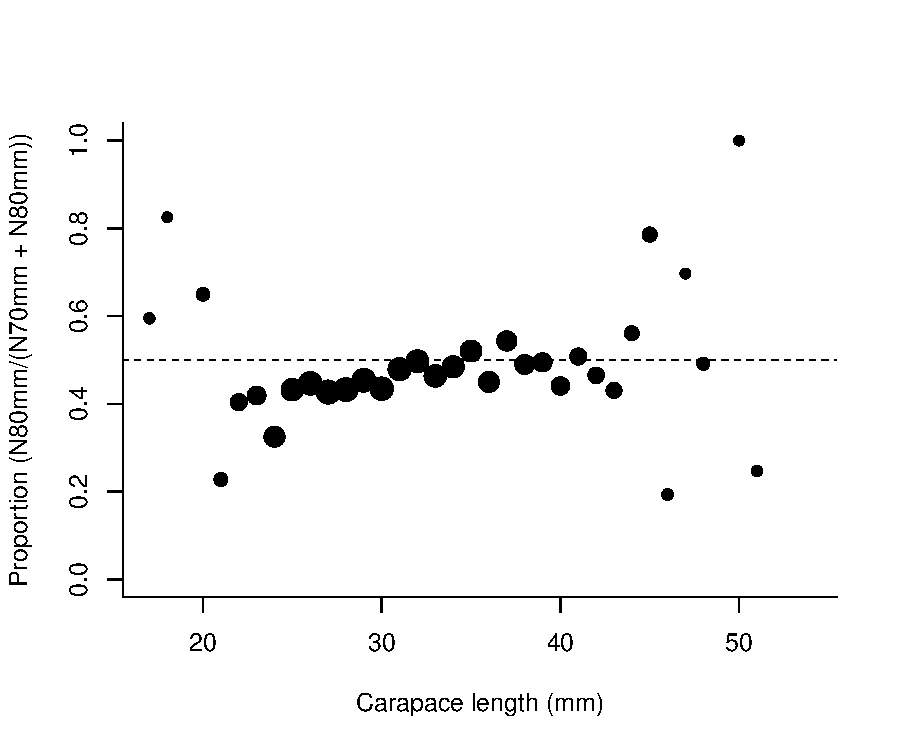
\includegraphics[width=\maxwidth]{figure/rawprops-1} \caption[Proportion of Nephrops raised numbers retained in the 80mm over the sum of the 80mm and 70mm meshes]{Proportion of Nephrops raised numbers retained in the 80mm over the sum of the 80mm and 70mm meshes.}\label{fig:rawprops}
\end{figure}


\end{knitrout}

\section{Models}
A catch comparison binomial Generalized Additive/Linear Mixed Model is suitable choice for these count data where we are interested in estimating how the proportion changes with carapace length. We first try a model with only carapace length as an explanatory variable with haul random effects.

\begin{knitrout}\footnotesize
\definecolor{shadecolor}{rgb}{0.969, 0.969, 0.969}\color{fgcolor}\begin{kframe}
\begin{alltt}
\hlkwd{library}\hlstd{(mgcv)}

\hlstd{neph.7080.cast}\hlopt{$}\hlstd{dum} \hlkwb{<-} \hlnum{1}

\hlcom{## no length effect}
\hlstd{gamm.null} \hlkwb{<-} \hlkwd{gam}\hlstd{(}\hlkwd{cbind}\hlstd{(mesh80mm_Count, mesh70mm_Count)} \hlopt{~} \hlnum{1} \hlopt{+}
                 \hlkwd{s}\hlstd{(fHAUL,} \hlkwc{bs}\hlstd{=}\hlstr{"re"}\hlstd{,} \hlkwc{by} \hlstd{= dum),}
                 \hlkwc{offset} \hlstd{=}
                 \hlkwd{log}\hlstd{(mesh80mm_Overall.Sampling.Ratio} \hlopt{/}
                     \hlstd{mesh70mm_Overall.Sampling.Ratio),}
                 \hlkwc{family} \hlstd{= binomial,}
                 \hlkwc{data} \hlstd{= neph.7080.cast)}

\hlstd{gamm.alt} \hlkwb{<-} \hlkwd{gam}\hlstd{(}\hlkwd{cbind}\hlstd{(mesh80mm_Count, mesh70mm_Count)} \hlopt{~}
                \hlkwd{s}\hlstd{(Carapace.length,} \hlkwc{k} \hlstd{=} \hlnum{5}\hlstd{)} \hlopt{+}
                \hlkwd{s}\hlstd{(fHAUL,} \hlkwc{bs}\hlstd{=}\hlstr{"re"}\hlstd{,} \hlkwc{by} \hlstd{= dum),}
                \hlkwc{offset} \hlstd{=}
                \hlkwd{log}\hlstd{(mesh80mm_Overall.Sampling.Ratio} \hlopt{/}
                    \hlstd{mesh70mm_Overall.Sampling.Ratio),}
                \hlkwc{family} \hlstd{= binomial,}
                \hlkwc{data} \hlstd{= neph.7080.cast)}

\hlcom{## likelihood ratio test for the significance of carapace length}
\hlkwd{anova}\hlstd{(gamm.null, gamm.alt,} \hlkwc{test} \hlstd{=} \hlstr{"Chisq"}\hlstd{)}
\end{alltt}
\begin{verbatim}
## Analysis of Deviance Table
## 
## Model 1: cbind(mesh80mm_Count, mesh70mm_Count) ~ 1 + s(fHAUL, bs = "re", 
##     by = dum)
## Model 2: cbind(mesh80mm_Count, mesh70mm_Count) ~ s(Carapace.length, k = 5) + 
##     s(fHAUL, bs = "re", by = dum)
##   Resid. Df Resid. Dev    Df Deviance Pr(>Chi)   
## 1       324        438                           
## 2       323        430 0.998     8.41   0.0037 **
## ---
## Signif. codes:  0 '***' 0.001 '**' 0.01 '*' 0.05 '.' 0.1 ' ' 1
\end{verbatim}
\end{kframe}
\end{knitrout}

Plot the predictions from this model.

\begin{knitrout}\footnotesize
\definecolor{shadecolor}{rgb}{0.969, 0.969, 0.969}\color{fgcolor}\begin{kframe}
\begin{alltt}
\hlstd{mean.catch} \hlkwb{<-} \hlkwd{mean}\hlstd{(}\hlkwd{c}\hlstd{(}\hlkwd{unique}\hlstd{(neph.7080.cast}\hlopt{$}\hlstd{mesh70mm_Total.catch),}
                     \hlkwd{unique}\hlstd{(neph.7080.cast}\hlopt{$}\hlstd{mesh80mm_Total.catch)))}

\hlcom{## data frame to predictfor}
\hlstd{pred.df} \hlkwb{<-} \hlkwd{data.frame}\hlstd{(}\hlkwc{Carapace.length} \hlstd{= cl.vec,}
                      \hlkwc{fHAUL} \hlstd{=} \hlstr{"H1"}\hlstd{,}
                      \hlkwc{dum} \hlstd{=} \hlnum{0}\hlstd{,}
                      \hlkwc{mesh80mm_Overall.Sampling.Ratio} \hlstd{=} \hlnum{1}\hlstd{,}
                      \hlkwc{mesh70mm_Overall.Sampling.Ratio} \hlstd{=} \hlnum{1}\hlstd{,}
                      \hlkwc{mesh70mm_Total.catch} \hlstd{= mean.catch,}
                      \hlkwc{mesh80mm_Total.catch} \hlstd{= mean.catch}
                      \hlstd{)}

\hlstd{pred.gamm.alt} \hlkwb{<-} \hlkwd{predict}\hlstd{(gamm.alt,} \hlkwc{newdata} \hlstd{= pred.df,} \hlkwc{se.fit} \hlstd{=} \hlnum{TRUE}\hlstd{)}

\hlcom{## predicted proportions and confidence intervals}
\hlstd{pred.df}\hlopt{$}\hlstd{pred.prop} \hlkwb{<-} \hlkwd{plogis}\hlstd{(pred.gamm.alt}\hlopt{$}\hlstd{fit)}
\hlstd{pred.df}\hlopt{$}\hlstd{lwr.prop} \hlkwb{<-} \hlkwd{plogis}\hlstd{(pred.gamm.alt}\hlopt{$}\hlstd{fit} \hlopt{-} \hlkwd{qnorm}\hlstd{(}\hlnum{0.975}\hlstd{)} \hlopt{*} \hlstd{pred.gamm.alt}\hlopt{$}\hlstd{se.fit)}
\hlstd{pred.df}\hlopt{$}\hlstd{upr.prop} \hlkwb{<-} \hlkwd{plogis}\hlstd{(pred.gamm.alt}\hlopt{$}\hlstd{fit} \hlopt{+} \hlkwd{qnorm}\hlstd{(}\hlnum{0.975}\hlstd{)} \hlopt{*} \hlstd{pred.gamm.alt}\hlopt{$}\hlstd{se.fit)}


\hlkwd{with}\hlstd{(count.df,} \hlkwd{plot}\hlstd{(Carapace.length, prop.80,} \hlkwc{ylim} \hlstd{=} \hlkwd{c}\hlstd{(}\hlnum{0}\hlstd{,} \hlnum{1}\hlstd{),} \hlkwc{pch} \hlstd{=} \hlnum{19}\hlstd{,}
                    \hlkwc{xlab} \hlstd{=} \hlstr{"Carapace length (mm)"}\hlstd{,}
                    \hlkwc{ylab} \hlstd{=} \hlstr{"Proportion (N80mm/(N70mm + N80mm))"}\hlstd{,}
                    \hlkwc{bty} \hlstd{=} \hlstr{"L"}\hlstd{))}

\hlkwd{with}\hlstd{(pred.df,} \hlkwd{lines}\hlstd{(Carapace.length, pred.prop))}
\hlkwd{with}\hlstd{(pred.df,} \hlkwd{lines}\hlstd{(Carapace.length, lwr.prop,} \hlkwc{lty} \hlstd{=} \hlnum{2}\hlstd{))}
\hlkwd{with}\hlstd{(pred.df,} \hlkwd{lines}\hlstd{(Carapace.length, upr.prop,} \hlkwc{lty} \hlstd{=} \hlnum{2}\hlstd{))}
\hlkwd{abline}\hlstd{(}\hlkwc{h} \hlstd{=} \hlnum{0.5}\hlstd{,} \hlkwc{col} \hlstd{=} \hlstr{"slategrey"}\hlstd{)}
\end{alltt}
\end{kframe}\begin{figure}
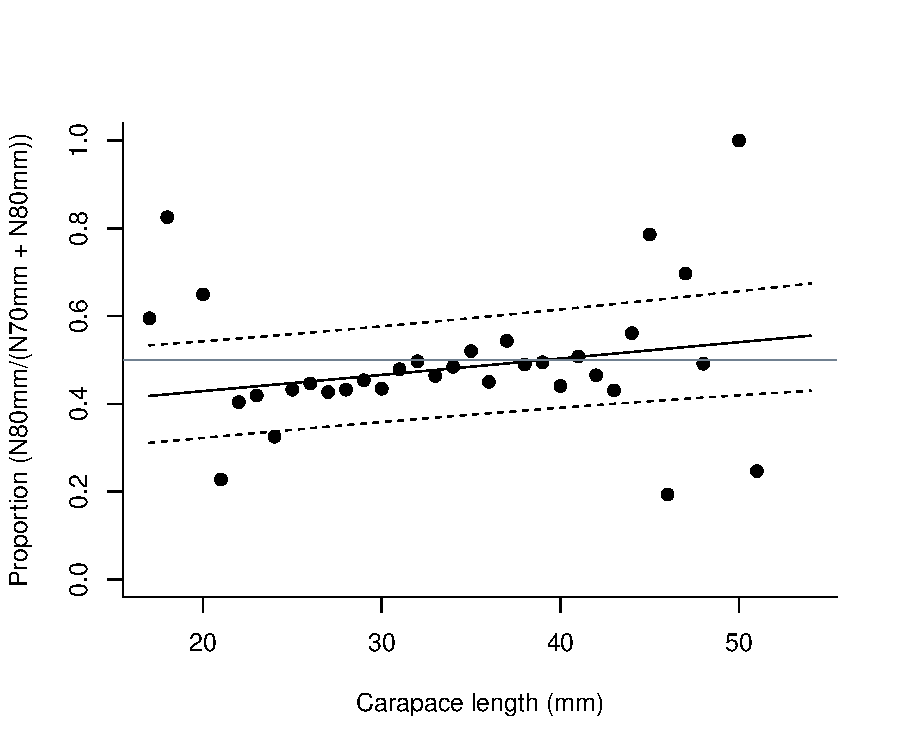
\includegraphics[width=\maxwidth]{figure/glmmsimple-1} \caption[Predicted proportion from binomial GLMM without covariates]{Predicted proportion from binomial GLMM without covariates.}\label{fig:glmmsimple}
\end{figure}


\end{knitrout}

The cause of the wide confidence intervals (Figure ~ \ref{fig:glmmsimple}) is the large amount of inter-haul variability in the proportion retained in the 80mm (Figure~\ref{fig:haulprop})

\begin{knitrout}\footnotesize
\definecolor{shadecolor}{rgb}{0.969, 0.969, 0.969}\color{fgcolor}\begin{kframe}
\begin{alltt}
\hlcom{## Get the proportion at length by haul}
\hlstd{haul.count.df} \hlkwb{<-} \hlkwd{expand.grid}\hlstd{(}\hlkwc{Carapace.length} \hlstd{= cl.vec,}
                             \hlkwc{fHAUL} \hlstd{=} \hlkwd{unique}\hlstd{(neph.7080.cast}\hlopt{$}\hlstd{fHAUL))}

\hlcom{## order the levels}
\hlstd{haul.count.df}\hlopt{$}\hlstd{fHAUL} \hlkwb{<-} \hlkwd{factor}\hlstd{(}\hlkwd{as.character}\hlstd{(haul.count.df}\hlopt{$}\hlstd{fHAUL),}
                              \hlkwc{levels} \hlstd{=} \hlkwd{c}\hlstd{(}\hlkwd{paste}\hlstd{(}\hlstr{"H"}\hlstd{,} \hlnum{1}\hlopt{:}\hlnum{12}\hlstd{,} \hlkwc{sep} \hlstd{=} \hlstr{""}\hlstd{),} \hlstr{"H14"}\hlstd{))}

\hlstd{haul.count.df}\hlopt{$}\hlstd{prop.80} \hlkwb{<-} \hlnum{NA}
\hlstd{haul.count.df}\hlopt{$}\hlstd{lwr} \hlkwb{<-} \hlnum{NA}
\hlstd{haul.count.df}\hlopt{$}\hlstd{upr} \hlkwb{<-} \hlnum{NA}

\hlkwa{for}\hlstd{(i} \hlkwa{in} \hlnum{1}\hlopt{:}\hlkwd{dim}\hlstd{(haul.count.df)[}\hlnum{1}\hlstd{])\{}
  \hlstd{sub.dat} \hlkwb{<-} \hlkwd{subset}\hlstd{(neph.7080.cast,}
                    \hlstd{Carapace.length} \hlopt{==} \hlstd{haul.count.df}\hlopt{$}\hlstd{Carapace.length[i]} \hlopt{&}
                    \hlstd{fHAUL} \hlopt{==} \hlstd{haul.count.df}\hlopt{$}\hlstd{fHAUL[i])}
  \hlcom{##}
  \hlcom{##if((sub.dat$mesh80mm_Raised.count + sub.dat$mesh70mm_Raised.count) > 0)\{}
  \hlkwa{if}\hlstd{(}\hlkwd{dim}\hlstd{(sub.dat)[}\hlnum{1}\hlstd{]} \hlopt{>} \hlnum{0}\hlstd{)\{}
    \hlstd{btest} \hlkwb{<-} \hlkwd{with}\hlstd{(sub.dat,}
                  \hlkwd{binom.test}\hlstd{(}\hlkwc{x} \hlstd{=} \hlkwd{round}\hlstd{(mesh80mm_Raised.count),}
                             \hlkwc{n} \hlstd{=} \hlkwd{round}\hlstd{(mesh80mm_Raised.count} \hlopt{+} \hlstd{mesh70mm_Raised.count)))}
    \hlcom{##}
    \hlstd{haul.count.df}\hlopt{$}\hlstd{prop.80[i]} \hlkwb{<-} \hlstd{btest}\hlopt{$}\hlstd{estimate}
    \hlstd{haul.count.df}\hlopt{$}\hlstd{lwr[i]} \hlkwb{<-} \hlstd{btest}\hlopt{$}\hlstd{conf.int[}\hlnum{1}\hlstd{]}
    \hlstd{haul.count.df}\hlopt{$}\hlstd{upr[i]} \hlkwb{<-} \hlstd{btest}\hlopt{$}\hlstd{conf.int[}\hlnum{2}\hlstd{]}
    \hlcom{##}
    \hlkwd{rm}\hlstd{(}\hlkwc{list} \hlstd{=} \hlkwd{c}\hlstd{(}\hlstr{"sub.dat"}\hlstd{,} \hlstr{"btest"}\hlstd{))}
  \hlstd{\}}
\hlstd{\}}

\hlcom{## get predictions at the HAUL level from model}
\hlstd{haul.count.df}\hlopt{$}\hlstd{dum} \hlkwb{<-} \hlnum{1}
\hlstd{haul.count.df}\hlopt{$}\hlstd{pred.prop} \hlkwb{<-} \hlkwd{plogis}\hlstd{(}\hlkwd{predict}\hlstd{(gamm.alt,} \hlkwc{newdata} \hlstd{= haul.count.df))}


\hlkwd{library}\hlstd{(ggplot2)}

\hlstd{blue2red} \hlkwb{<-} \hlkwd{colorRampPalette}\hlstd{(}\hlkwd{c}\hlstd{(}\hlstr{"darkblue"}\hlstd{,} \hlstr{"white"}\hlstd{,} \hlstr{"red"}\hlstd{))}

\hlkwd{ggplot}\hlstd{(haul.count.df,} \hlkwd{aes}\hlstd{(}\hlkwc{x} \hlstd{= Carapace.length,} \hlkwc{y} \hlstd{= prop.80))} \hlopt{+}
  \hlkwd{geom_point}\hlstd{(}\hlkwd{aes}\hlstd{(}\hlkwc{colour} \hlstd{= fHAUL))} \hlopt{+}
  \hlkwd{geom_line}\hlstd{(}\hlkwc{data} \hlstd{= haul.count.df,} \hlkwd{aes}\hlstd{(}\hlkwc{x} \hlstd{= Carapace.length,} \hlkwc{y} \hlstd{= pred.prop,}  \hlkwc{colour} \hlstd{= fHAUL))} \hlopt{+}
  \hlkwd{scale_colour_manual}\hlstd{(}\hlkwc{values} \hlstd{=} \hlkwd{blue2red}\hlstd{(}\hlnum{13}\hlstd{))} \hlopt{+} \hlkwd{ylab}\hlstd{(}\hlstr{"Proportion in 80mm"}\hlstd{)}
\end{alltt}


{\ttfamily\noindent\color{warningcolor}{\#\# Warning: Removed 118 rows containing missing values (geom\_point).}}\end{kframe}\begin{figure}
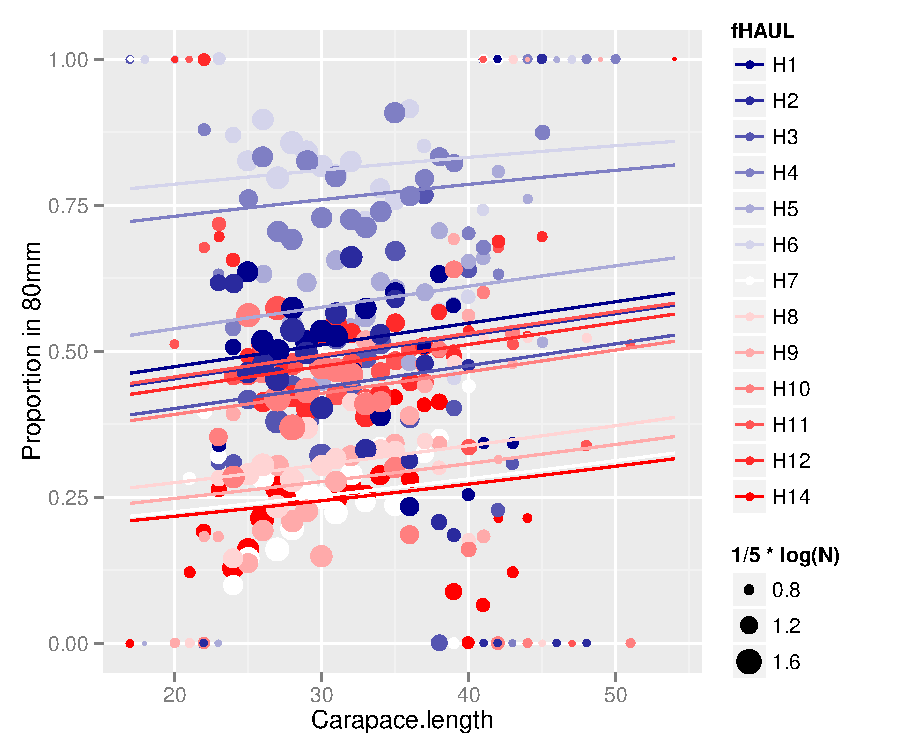
\includegraphics[width=\maxwidth]{figure/haulprop-1} \caption[Observed proportion in the 80mm by haul]{Observed proportion in the 80mm by haul. Note the wide variability of the proportion with some having much higher or lower proportions. Fitted lines come from the GLMM with carapace length only.}\label{fig:haulprop}
\end{figure}


\end{knitrout}

We can take a look at additional measured covariates to see if these relate to the haul-level variability (random effects in the model above) (Figure~\ref{fig:ranefplots}).

\begin{knitrout}\footnotesize
\definecolor{shadecolor}{rgb}{0.969, 0.969, 0.969}\color{fgcolor}\begin{kframe}
\begin{alltt}
\hlcom{##}
\hlstd{ranef.df} \hlkwb{<-} \hlkwd{data.frame}\hlstd{(}\hlkwc{fHAUL} \hlstd{=} \hlkwd{levels}\hlstd{(neph.7080.cast}\hlopt{$}\hlstd{fHAUL),}
                       \hlkwc{ranef} \hlstd{=} \hlkwd{coef}\hlstd{(gamm.alt)[}\hlopt{-}\hlkwd{c}\hlstd{(}\hlnum{1}\hlopt{:}\hlnum{5}\hlstd{)])}
\hlcom{##}
\hlstd{covar.names} \hlkwb{<-} \hlkwd{c}\hlstd{(}\hlstr{"fHAUL"}\hlstd{,} \hlstr{"mesh70mm_Net.position"}\hlstd{,} \hlstr{"mesh70mm_Total.catch"}\hlstd{,}
                 \hlstr{"mesh80mm_Net.position"}\hlstd{,} \hlstr{"mesh80mm_Total.catch"}\hlstd{)}
\hlcom{##}
\hlstd{covar.df} \hlkwb{<-} \hlkwd{unique}\hlstd{(neph.7080.cast[, covar.names])}
\hlcom{##}
\hlstd{ranef.df} \hlkwb{<-} \hlkwd{merge}\hlstd{(ranef.df, covar.df)}
\hlcom{## convert to long format for plotting}
\hlstd{ranef.df} \hlkwb{<-} \hlkwd{melt}\hlstd{(ranef.df,} \hlkwc{id} \hlstd{=} \hlkwd{c}\hlstd{(}\hlstr{"fHAUL"}\hlstd{,} \hlstr{"ranef"}\hlstd{))}
\hlcom{##}
\hlkwd{ggplot}\hlstd{(ranef.df,} \hlkwd{aes}\hlstd{(}\hlkwc{x} \hlstd{= value,} \hlkwc{y} \hlstd{= ranef))} \hlopt{+}
  \hlkwd{geom_point}\hlstd{()} \hlopt{+}
  \hlkwd{facet_wrap}\hlstd{(}\hlopt{~} \hlstd{variable,} \hlkwc{scales} \hlstd{=} \hlstr{"free"}\hlstd{)} \hlopt{+}
  \hlkwd{xlab}\hlstd{(}\hlstr{"Covariate value"}\hlstd{)} \hlopt{+}
  \hlkwd{ylab}\hlstd{(}\hlstr{"Random effect"}\hlstd{)}
\end{alltt}
\end{kframe}\begin{figure}
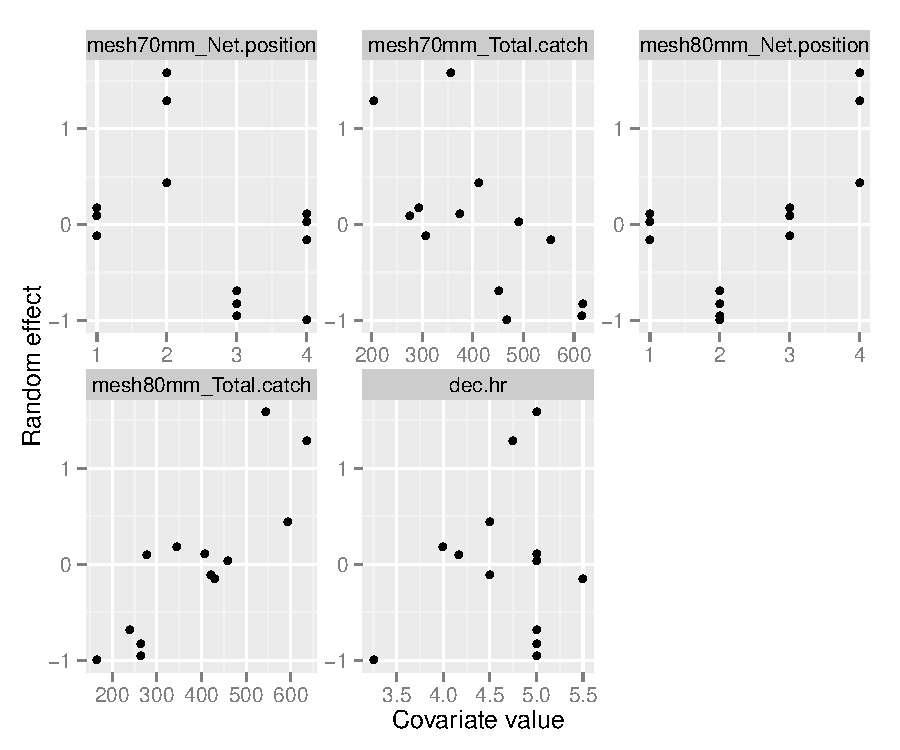
\includegraphics[width=\maxwidth]{figure/ranefplots-1} \caption[Relationship between the random effects of the carapace length only model and measured covariates ]{Relationship between the random effects of the carapace length only model and measured covariates .}\label{fig:ranefplots}
\end{figure}


\end{knitrout}

There are some strong relationships between the random effects and measured covariates (Figure~\ref{fig:ranefplots}). It is best to include these measured variables in the model as fixed effects.

\begin{knitrout}\footnotesize
\definecolor{shadecolor}{rgb}{0.969, 0.969, 0.969}\color{fgcolor}\begin{kframe}
\begin{alltt}
\hlcom{## including additional covariates}
\hlcom{## check identifiability}
\hlstd{neph.7080.cast}\hlopt{$}\hlstd{fmesh80mm_Net.position} \hlkwb{<-}
  \hlkwd{factor}\hlstd{(}\hlkwd{paste}\hlstd{(}\hlstr{"pos"}\hlstd{,}
               \hlstd{neph.7080.cast}\hlopt{$}\hlstd{mesh80mm_Net.position,} \hlkwc{sep} \hlstd{=} \hlstr{""}\hlstd{))}

\hlcom{## using log of total catch weights - return to this}
\hlstd{neph.7080.cast}\hlopt{$}\hlstd{log.mesh80mm_Total.catch} \hlkwb{<-} \hlkwd{log}\hlstd{(neph.7080.cast}\hlopt{$}\hlstd{mesh80mm_Total.catch)}
\hlstd{neph.7080.cast}\hlopt{$}\hlstd{log.mesh70mm_Total.catch} \hlkwb{<-} \hlkwd{log}\hlstd{(neph.7080.cast}\hlopt{$}\hlstd{mesh70mm_Total.catch)}

\hlcom{## Note should return to this warning later}
\hlcom{## fits okay in gam but glmm used for effects package}
\hlstd{glmm.alt.covar} \hlkwb{<-} \hlkwd{glmer}\hlstd{(}\hlkwd{cbind}\hlstd{(mesh80mm_Count, mesh70mm_Count)} \hlopt{~}
                        \hlcom{##I(log(mesh80mm_Total.catch / mesh70mm_Total.catch)) * Carapace.length +}
                        \hlstd{log.mesh80mm_Total.catch} \hlopt{+} \hlstd{log.mesh70mm_Total.catch} \hlopt{+}
                        \hlstd{Carapace.length} \hlopt{+}
                        \hlstd{fmesh80mm_Net.position} \hlopt{+}
                        \hlstd{(}\hlnum{1} \hlopt{|} \hlstd{fHAUL),}
                        \hlkwc{offset} \hlstd{=}
                        \hlkwd{log}\hlstd{(mesh80mm_Overall.Sampling.Ratio} \hlopt{/}
                            \hlstd{mesh70mm_Overall.Sampling.Ratio),}
                        \hlkwc{family} \hlstd{= binomial,}
                        \hlkwc{data} \hlstd{= neph.7080.cast)}
\end{alltt}


{\ttfamily\noindent\color{warningcolor}{\#\# Warning in checkConv(attr(opt, "{}derivs"{}), opt\$par, ctrl = control\$checkConv, : Model failed to converge with max|grad| = 0.00492158 (tol = 0.001, component 2)}}

{\ttfamily\noindent\color{warningcolor}{\#\# Warning in checkConv(attr(opt, "{}derivs"{}), opt\$par, ctrl = control\$checkConv, : Model is nearly unidentifiable: large eigenvalue ratio\\\#\#\ \ - Rescale variables?}}\begin{alltt}
\hlcom{## use effects package to get prediction for model with net position}
\hlcom{## set predictor variables}
\hlstd{xlevels} \hlkwb{<-} \hlkwd{list}\hlstd{(}\hlkwc{Carapace.length} \hlstd{= cl.vec}
                \hlcom{##mesh80mm_Total.catch = mean.catch,}
                \hlcom{##mesh70mm_Total.catch = mean.catch}
                \hlstd{)}
\hlcom{## if we wanted to set the proportions of net positions equivalent}
\hlcom{## otherwise set to the proportion observed in the data}
\hlcom{##given.values <- c("fmesh80mm_Net.positionpos2" = 1/4,}
\hlcom{##                  "fmesh80mm_Net.positionpos3" = 1/4,}
\hlcom{##                  "fmesh80mm_Net.positionpos4" = 1/4}
\hlcom{##                  )}

\hlcom{##cl.effect <- effect("Carapace.length", glmm.alt.covar, xlevels = xlevels, offset = 0, given.values = given.values)}
\hlstd{cl.effect} \hlkwb{<-} \hlkwd{effect}\hlstd{(}\hlstr{"Carapace.length"}\hlstd{, glmm.alt.covar,} \hlkwc{xlevels} \hlstd{= xlevels,} \hlkwc{offset} \hlstd{=} \hlnum{0}\hlstd{)}
\end{alltt}
\end{kframe}
\end{knitrout}

Finally plot the effect of carapace length with the other variables set to their mean in the data (Figure~\ref{fig:glmmcovar}).

\begin{knitrout}\footnotesize
\definecolor{shadecolor}{rgb}{0.969, 0.969, 0.969}\color{fgcolor}\begin{kframe}
\begin{alltt}
\hlkwd{with}\hlstd{(count.df,} \hlkwd{plot}\hlstd{(Carapace.length, prop.80,} \hlkwc{ylim} \hlstd{=} \hlkwd{c}\hlstd{(}\hlnum{0}\hlstd{,} \hlnum{1}\hlstd{),} \hlkwc{pch} \hlstd{=} \hlnum{19}\hlstd{,}
                    \hlkwc{xlab} \hlstd{=} \hlstr{"Carapace length (mm)"}\hlstd{,}
                    \hlkwc{ylab} \hlstd{=} \hlstr{"Proportion (N80mm/(N70mm + N80mm))"}\hlstd{,}
                    \hlkwc{bty} \hlstd{=} \hlstr{"L"}\hlstd{))}

\hlcom{## effects prediction}
\hlkwd{lines}\hlstd{(cl.vec,} \hlkwd{plogis}\hlstd{(cl.effect}\hlopt{$}\hlstd{fit[,} \hlnum{1}\hlstd{]))}
\hlkwd{lines}\hlstd{(cl.vec,} \hlkwd{plogis}\hlstd{(cl.effect}\hlopt{$}\hlstd{lower[,} \hlnum{1}\hlstd{]),} \hlkwc{lty} \hlstd{=} \hlnum{2}\hlstd{)}
\hlkwd{lines}\hlstd{(cl.vec,} \hlkwd{plogis}\hlstd{(cl.effect}\hlopt{$}\hlstd{upper[,} \hlnum{1}\hlstd{]),} \hlkwc{lty} \hlstd{=} \hlnum{2}\hlstd{)}
\hlkwd{abline}\hlstd{(}\hlkwc{h} \hlstd{=} \hlnum{0.5}\hlstd{,} \hlkwc{col} \hlstd{=} \hlstr{"slategrey"}\hlstd{)}
\end{alltt}
\end{kframe}\begin{figure}
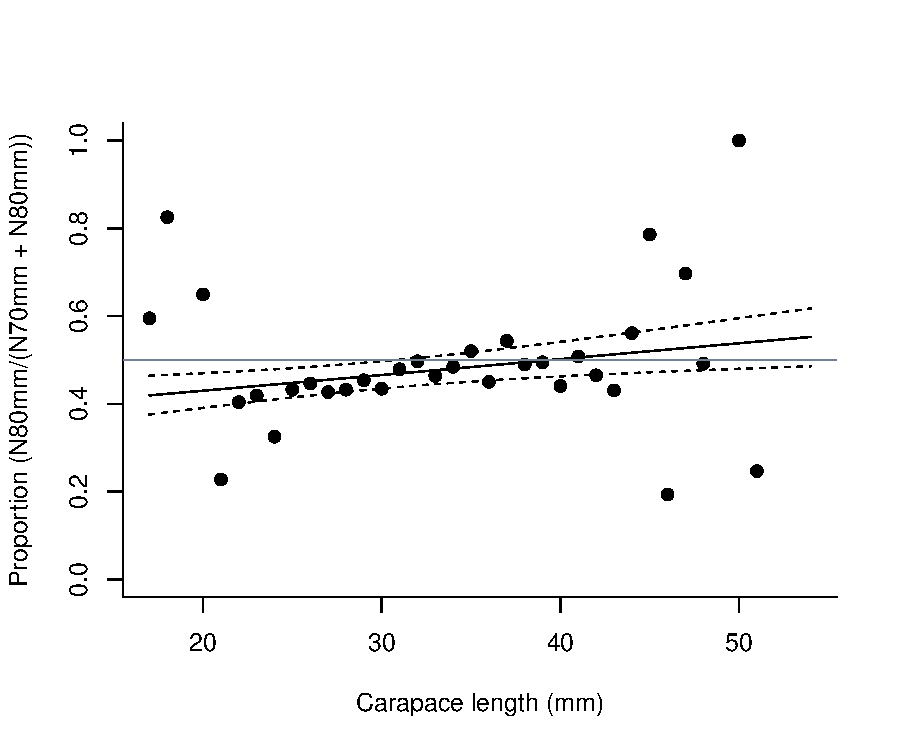
\includegraphics[width=\maxwidth]{figure/glmmcovar-1} \caption[Predicted proportion from binomial GLMM with covariates]{Predicted proportion from binomial GLMM with covariates. Note in the predictions the bulk weights are set to their mean and the net positions to their proportional occurence in the data.}\label{fig:glmmcovar}
\end{figure}


\end{knitrout}

Finally test length effect in covariate model
\begin{knitrout}\footnotesize
\definecolor{shadecolor}{rgb}{0.969, 0.969, 0.969}\color{fgcolor}\begin{kframe}
\begin{alltt}
\hlstd{glmm.alt.covar.nolength} \hlkwb{<-} \hlkwd{glmer}\hlstd{(}\hlkwd{cbind}\hlstd{(mesh80mm_Count, mesh70mm_Count)} \hlopt{~}
                        \hlstd{log.mesh80mm_Total.catch} \hlopt{+} \hlstd{log.mesh70mm_Total.catch} \hlopt{+}
                        \hlstd{fmesh80mm_Net.position} \hlopt{+}
                        \hlstd{(}\hlnum{1} \hlopt{|} \hlstd{fHAUL),}
                        \hlkwc{offset} \hlstd{=}
                        \hlkwd{log}\hlstd{(mesh80mm_Overall.Sampling.Ratio} \hlopt{/}
                            \hlstd{mesh70mm_Overall.Sampling.Ratio),}
                        \hlkwc{family} \hlstd{= binomial,}
                        \hlkwc{data} \hlstd{= neph.7080.cast)}

\hlcom{## likelihood ratio test}
\hlkwd{anova}\hlstd{(glmm.alt.covar.nolength, glmm.alt.covar)}
\end{alltt}
\begin{verbatim}
## Data: neph.7080.cast
## Models:
## glmm.alt.covar.nolength: cbind(mesh80mm_Count, mesh70mm_Count) ~ log.mesh80mm_Total.catch + 
## glmm.alt.covar.nolength:     log.mesh70mm_Total.catch + fmesh80mm_Net.position + (1 | 
## glmm.alt.covar.nolength:     fHAUL)
## glmm.alt.covar: cbind(mesh80mm_Count, mesh70mm_Count) ~ log.mesh80mm_Total.catch + 
## glmm.alt.covar:     log.mesh70mm_Total.catch + Carapace.length + fmesh80mm_Net.position + 
## glmm.alt.covar:     (1 | fHAUL)
##                         Df  AIC  BIC logLik deviance Chisq Chi Df
## glmm.alt.covar.nolength  7 1421 1448   -703     1407             
## glmm.alt.covar           8 1415 1445   -699     1399  8.09      1
##                         Pr(>Chisq)   
## glmm.alt.covar.nolength              
## glmm.alt.covar              0.0044 **
## ---
## Signif. codes:  0 '***' 0.001 '**' 0.01 '*' 0.05 '.' 0.1 ' ' 1
\end{verbatim}
\begin{alltt}
\hlcom{## significant effect of carapace length}
\end{alltt}
\end{kframe}
\end{knitrout}

\bibliography{../../../../misc/epif_bibliography}
\bibliographystyle{../../../../misc/cjfas}
\end{document}

